% \documentclass{beamer}
\documentclass[aspectratio=169]{beamer}
\usepackage{babel, graphicx}

\usepackage{tikz}
\usepackage[T1]{fontenc}
\usepackage{caption}
\usetheme{Frankfurt}

\title{ \large{Rock-Paper-Scissors} \\ 
        \small{ML 2023/2024}}

\author{
    Maksymilian Wiśniewski \and
    \textbf{(Michał Mękarski)} \\ \and
    Patryk Maciąg  \and
    Stanisław Reda
}

\date{}

\titlegraphic{
\centering
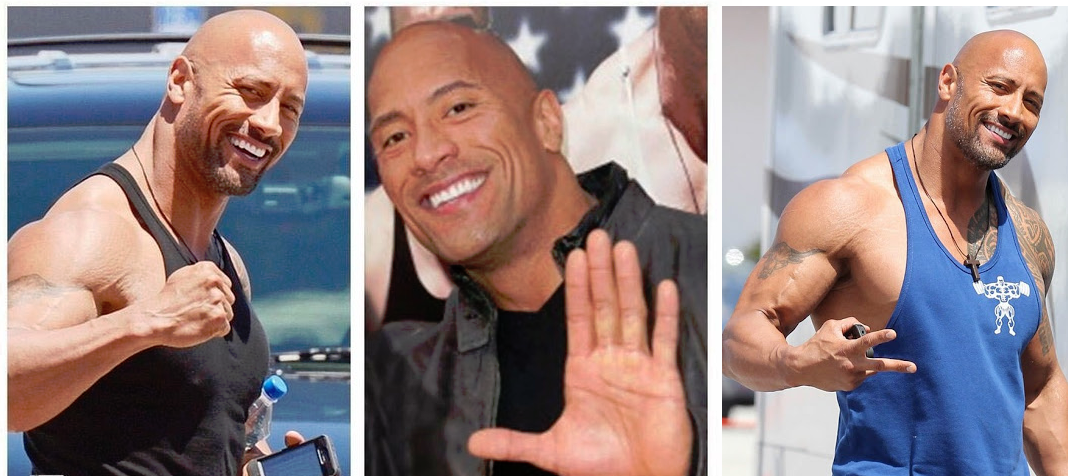
\includegraphics[height=1in, width=3in]{images/rock.png}
% 
\includegraphics[height=1in, width=3in]{images/cursed_elmo.jpg}
% 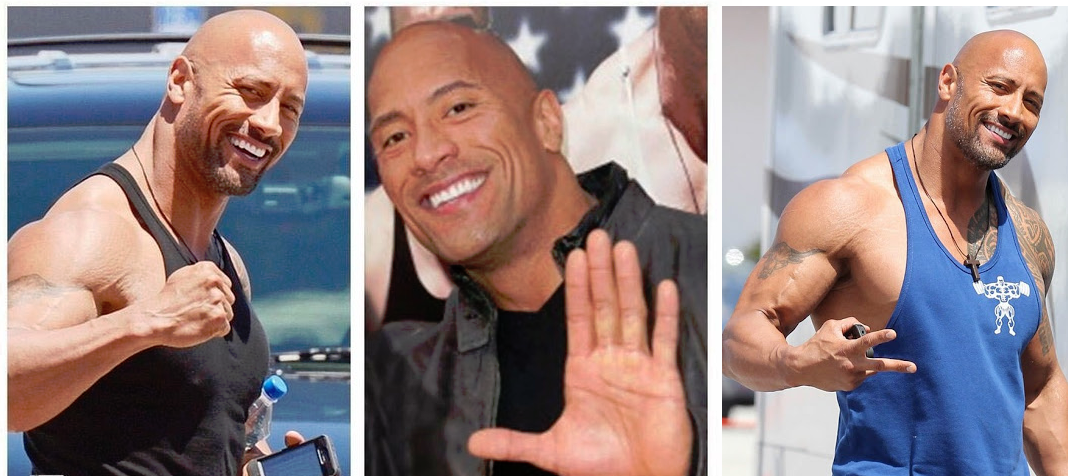
\includegraphics[height=1.5in, width=4in]{images/obraz.png}
}




\begin{document}


\maketitle





\section{Main Goal}

\begin{frame}
    \frametitle{Main Goal}
    \begin{itemize}
        \item We decided to focus on the classification of images.

        \item Our main goal is to classify the gesture in the photo as one of the three movements from the "Rock-Paper-Scissors" game with best possible accuracy.

        \item We want to see how far we can go with the tools learned in the lecture and compare the results obtained.
        
    \end{itemize}

\end{frame}


\section{Data}




\begin{frame}
    \frametitle{Data}
    Our dataset on Kaggle: \href{https://www.kaggle.com/datasets/drgfreeman/rockpaperscissors}{Rock-Paper-Scissors Images}
    
    \begin{figure}
    \centering
    \subfloat{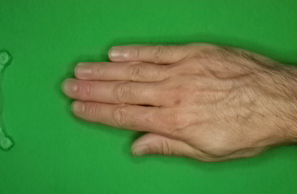
\includegraphics[width=0.3\textwidth, height=0.2\textheight]{images/img1.png}\label{fig:img1}}\hfill
    \subfloat{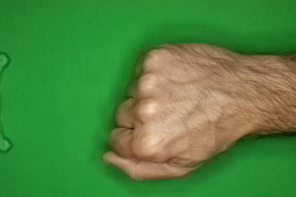
\includegraphics[width=0.3\textwidth, height=0.2\textheight]{images/img2.png}\label{fig:img2}}\hfill
    \subfloat{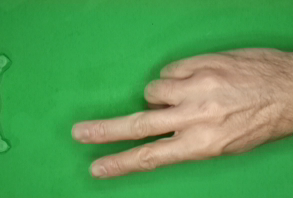
\includegraphics[width=0.3\textwidth, height=0.2\textheight]{images/img3.png}\label{fig:img3}}
    \end{figure}

    \begin{figure}
    \centering
    \subfloat{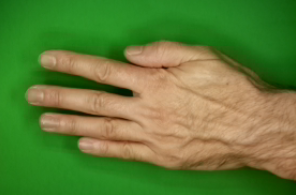
\includegraphics[width=0.3\textwidth, height=0.2\textheight]{images/img4.png}\label{fig:img1}}\hfill
    \subfloat{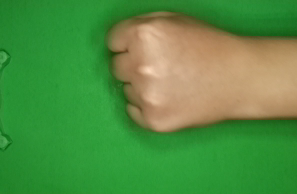
\includegraphics[width=0.3\textwidth, height=0.2\textheight]{images/img5.png}\label{fig:img2}}\hfill
    \subfloat{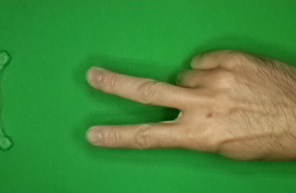
\includegraphics[width=0.3\textwidth, height=0.2\textheight]{images/img6.png}\label{fig:img3}}
    \end{figure}

    \begin{figure}
    \centering
    \subfloat{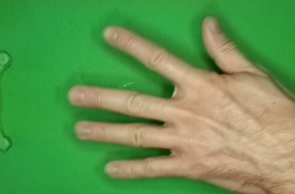
\includegraphics[width=0.3\textwidth, height=0.2\textheight]{images/img7.png}\label{fig:img1}}\hfill
    \subfloat{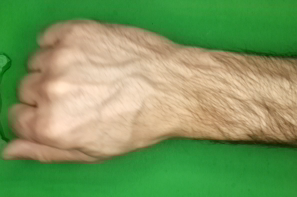
\includegraphics[width=0.3\textwidth, height=0.2\textheight]{images/img8.png}\label{fig:img2}}\hfill
    \subfloat{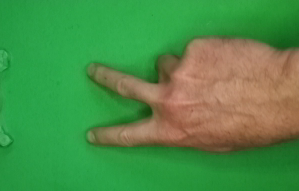
\includegraphics[width=0.3\textwidth, height=0.2\textheight]{images/img9.png}\label{fig:img3}}
    \end{figure}

\end{frame}


\section{Methods}

    
\begin{frame}

    \frametitle{Preprocessing}
\begin{center}

    \begin{itemize}
        \item Grayscale
        \item Normalization
        \item Pca
        
    \end{itemize}
\end{center}

\end{frame}




\begin{frame}
  \frametitle{PCA features}
\centering
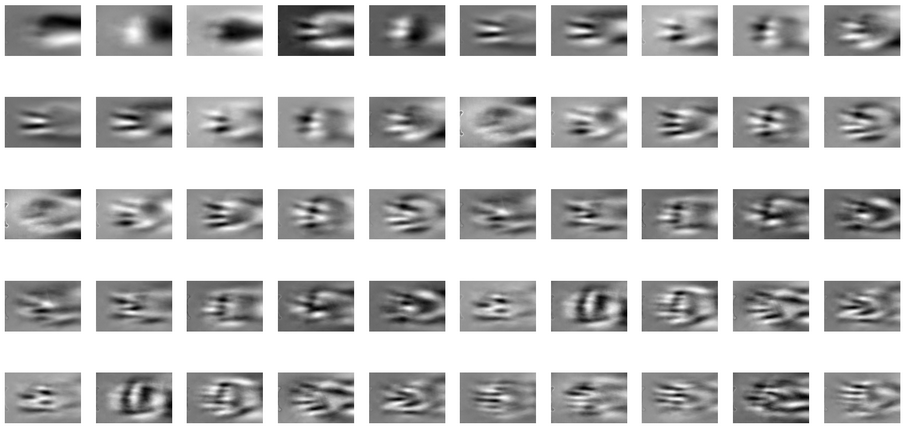
\includegraphics[scale=0.35]{images/simplepca.png}
\end{frame}








\begin{frame}
  \frametitle{No augmentation}

  \begin{table}
    \centering
    \captionsetup{labelformat=empty}
    \caption{KNN}
    \begin{tabular}{|c|c|c|c|}
    \hline
       & Mean & Std & Test \\
      \hline
      \textbf{Full imgs} & 91.14\% & 1.7\%  & 92.24\% \\
      \hline
      \textbf{Scaled imgs} & 91.48\% & 1.85\% & 92.46\% \\
      \hline
      \textbf{PCA} & 91.65\% & 2.26\% & 93.15\% \\
      \hline
    \end{tabular}
  \end{table}

  \begin{table}
    \centering
    \captionsetup{labelformat=empty}
    \caption{Decision tree}
    \begin{tabular}{|c|c|c|c|}
    \hline
       & Mean & Std & Test \\
      \hline
      \textbf{Scaled imgs} & 82.28\% & 3.91\% & 84.93\% \\
      \hline
      \textbf{PCA} & 76.00\% & 2.58\% & 78.99\% \\
      \hline
    \end{tabular}
  \end{table}

\end{frame}




\begin{frame}
  \frametitle{No augmentation}

  \begin{table}
    \centering
    \captionsetup{labelformat=empty}
    \caption{Random forest}
    \begin{tabular}{|c|c|c|c|}
    \hline
       & Mean & Std & Test \\
      \hline
      \textbf{Scaled imgs} & 94.28\% & 1.81\% & 95.43\% \\
      \hline
      \textbf{PCA} & 88.23\% & 2.15\% & 92.01\% \\
      \hline
    \end{tabular}
  \end{table}

  \begin{table}
    \centering
    \captionsetup{labelformat=empty}
    \caption{XGBoost}
    \begin{tabular}{|c|c|c|c|}
    \hline
       & Mean & Std & Test \\
      \hline
      \textbf{PCA} & 91.37\% & 1.29\% & 94.06\% \\
      \hline
    \end{tabular}
  \end{table}


  \begin{table}
    \centering
    \captionsetup{labelformat=empty}
    \caption{Support Vector Machine}
    \begin{tabular}{|c|c|c|c|}
    \hline
       & Mean & Std & Test \\
      \hline
      \textbf{PCA} & 93.88\% & 0.92\% & 94.75\% \\
      \hline
    \end{tabular}
  \end{table}

  

\end{frame}









\begin{frame}
  \frametitle{Augmented dataset}
\centering
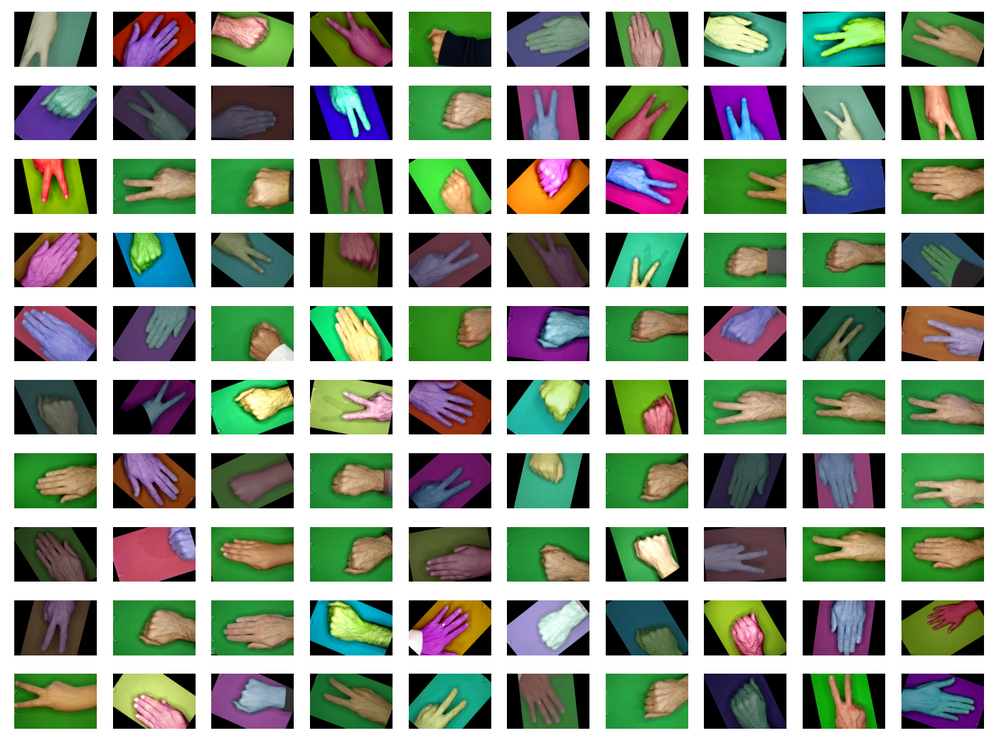
\includegraphics[height=0.85\textheight, width=0.9\textwidth]{images/augmented.png}
\end{frame}


\begin{frame}
  \frametitle{PCA features of augmented dataset}
\centering
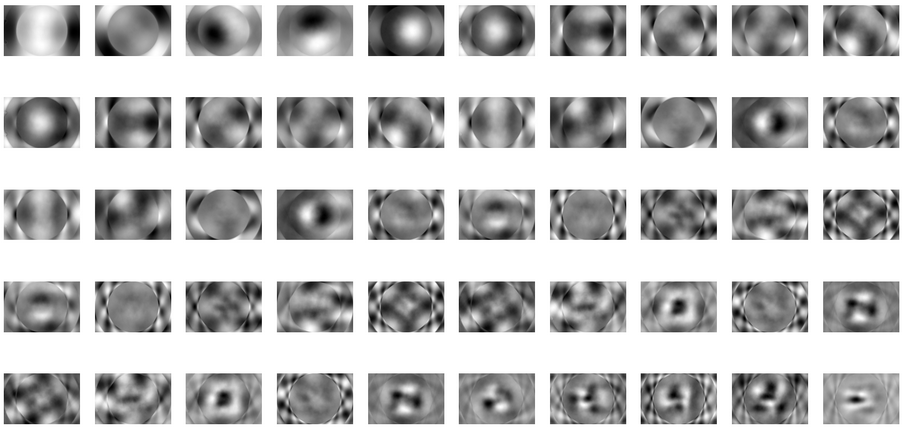
\includegraphics[height=0.7\textheight]{images/augmentedpca.png}
\end{frame}


\begin{frame}
    \frametitle{Feature extraction}
    \begin{itemize}
        \item We've used technique called transfer learning. 
        \item In which we deleted the \textit{softmax}  layer (i.e last layer) of pretrained neural network \textbf{VGG16}, for some further future extraction.
        
    \end{itemize}

\end{frame}


\begin{frame}
  \frametitle{Augmented dataset}
  \begin{table}
    \centering
    \captionsetup{labelformat=empty}
    \caption{KNN}
    \begin{tabular}{|c|c|c|c|}
    \hline
       & Mean & Std & Test \\
      \hline
      \textbf{Scaled imgs} & 69.13\% & 1.54\% & 71.67\% \\
      \hline
      \textbf{PCA} & 69.97\% & 1.25\% & 72.53\% \\
      \hline
      \textbf{VGG16} & 93.57\% & 0.91\% & 94.11\% \\
      \hline
    \end{tabular}
  \end{table}
  \begin{table}
    \centering
    \captionsetup{labelformat=empty}
    \caption{Decision tree}
    \begin{tabular}{|c|c|c|c|}
    \hline
       & Mean & Std & Test \\
      \hline
      \textbf{PCA} & 56.99\% & 2.39\% & 59.68\% \\
      \hline
      \textbf{VGG16} & 79.00\% & 1.40\% & 79.61\% \\
      \hline
    \end{tabular}
  \end{table}
\end{frame}
\begin{frame}
  \frametitle{Augmented dataset}

  \begin{table}
    \centering
    \captionsetup{labelformat=empty}
    \caption{Random forest}
    \begin{tabular}{|c|c|c|c|}
    \hline
       & Mean & Std & Test \\
      \hline
      \textbf{PCA} & 75.64\% & 1.62\% & 76.35\% \\
      \hline
      \textbf{VGG16} & 93.21\% & 1.00\% & 93.83\% \\
      \hline
    \end{tabular}
  % \end{table}

  % \begin{table}
    \centering
    \captionsetup{labelformat=empty}
    \caption{XGBoost}
    \begin{tabular}{|c|c|c|c|}
    \hline
       & Mean & Std & Test \\
      \hline
      \textbf{PCA} & 86.57\% & 1.09\% & 86.52\% \\
      \hline
      \textbf{VGG16} & 96.82\% & 0.92\% & 96.80\% \\
      \hline
    \end{tabular}
  % \end{table}


  % \begin{table}
    \centering
    \captionsetup{labelformat=empty}
    \caption{Support Vector Machine}
    \begin{tabular}{|c|c|c|c|}
    \hline
       & Mean & Std & Test \\
      \hline
      \textbf{PCA} & 77.37\% & 1.12\% & 79.38\% \\
      \hline
      \textbf{VGG16} & 98.42\% & 0.40\% & 98.11\% \\
      \hline
    \end{tabular}
  \end{table}

  

\end{frame}







\begin{frame}
  \frametitle{Contours-only dataset (using OpenCV, FAIL)}
\centering
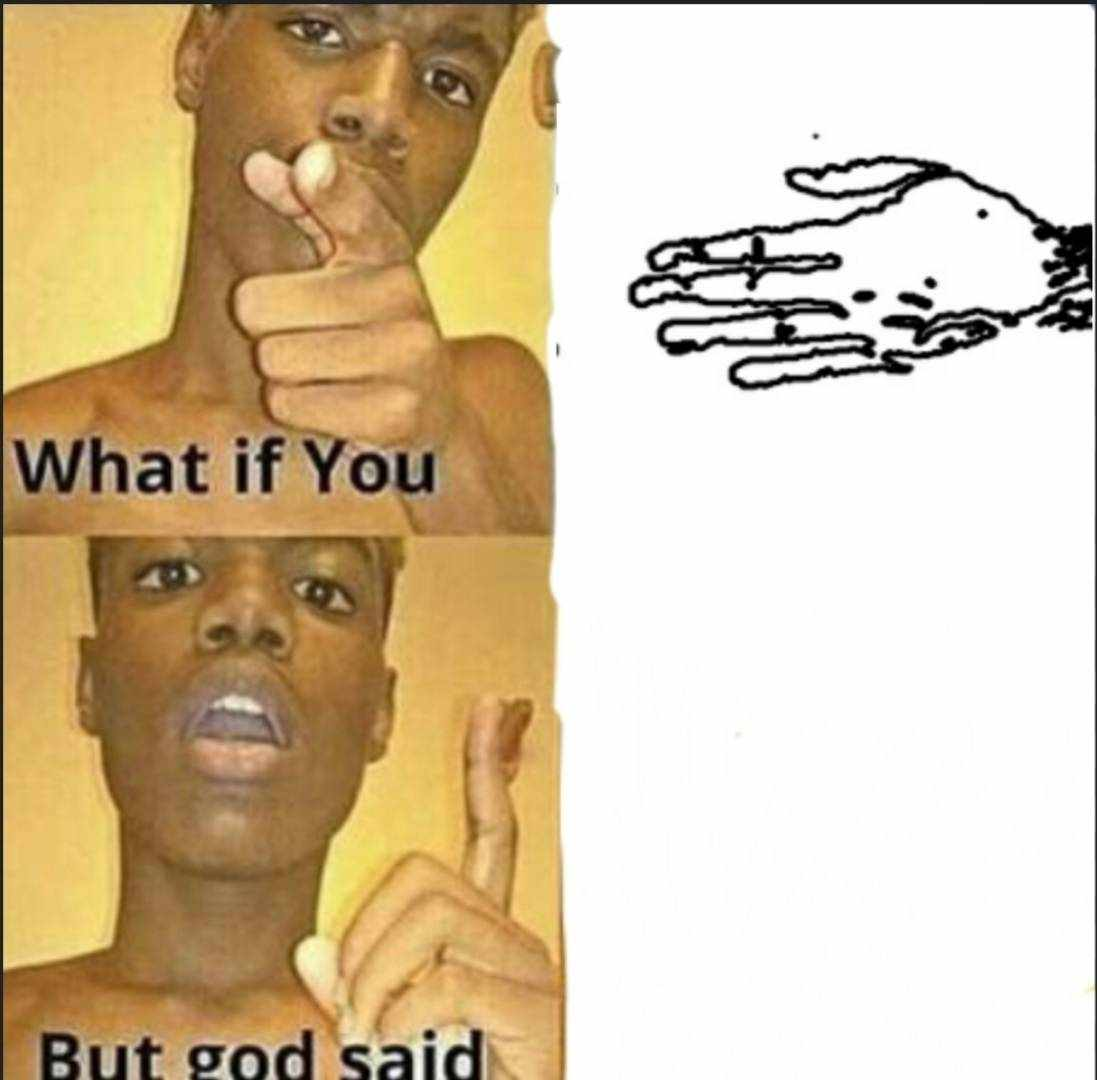
\includegraphics[height=0.87\textheight]{images/meme.png}
\end{frame}


\begin{frame}
  \frametitle{Contours-only dataset (using OpenCV, FAIL)}
\centering
\begin{figure}
    \centering
    \subfloat{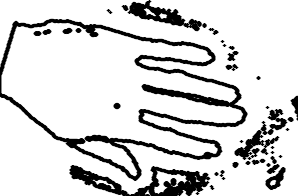
\includegraphics[width=0.3\textwidth, height=0.2\textheight]{images/contour1.png}\label{fig:img1}}\hfill
    \subfloat{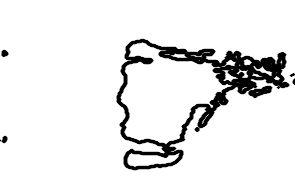
\includegraphics[width=0.3\textwidth, height=0.2\textheight]{images/contour2.png}\label{fig:img2}}\hfill
    \subfloat{
\includegraphics[width=0.3\textwidth, height=0.2\textheight]{images/contour3.png}\label{fig:img3}}
    \end{figure}

    \begin{figure}
    \centering
    \subfloat{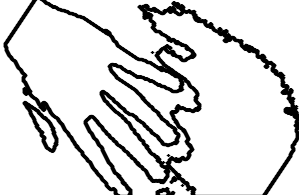
\includegraphics[width=0.3\textwidth, height=0.2\textheight]{images/contour4.png}\label{fig:img1}}\hfill
    \subfloat{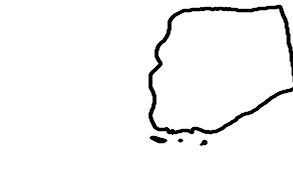
\includegraphics[width=0.3\textwidth, height=0.2\textheight]{images/contour5.png}\label{fig:img2}}\hfill
    \subfloat{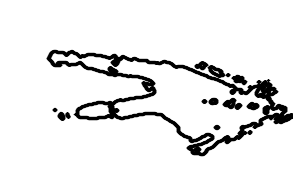
\includegraphics[width=0.3\textwidth, height=0.2\textheight]{images/contour6.png}\label{fig:img3}}
    \end{figure}

    \begin{figure}
    \centering
    \subfloat{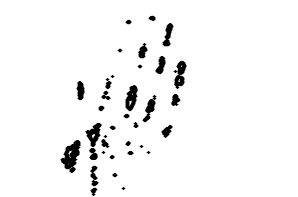
\includegraphics[width=0.3\textwidth, height=0.2\textheight]{images/contour7.png}\label{fig:img1}}\hfill
    \subfloat{
\includegraphics[width=0.3\textwidth, height=0.2\textheight]{images/contour8.png}\label{fig:img2}}\hfill
    \subfloat{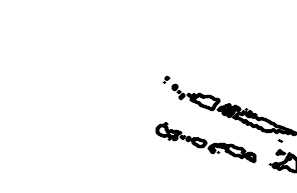
\includegraphics[width=0.3\textwidth, height=0.2\textheight]{images/contour9.png}\label{fig:img3}}
    \end{figure}
\end{frame}











\begin{frame}
  \frametitle{Self-made photos of hands}
  \centering
  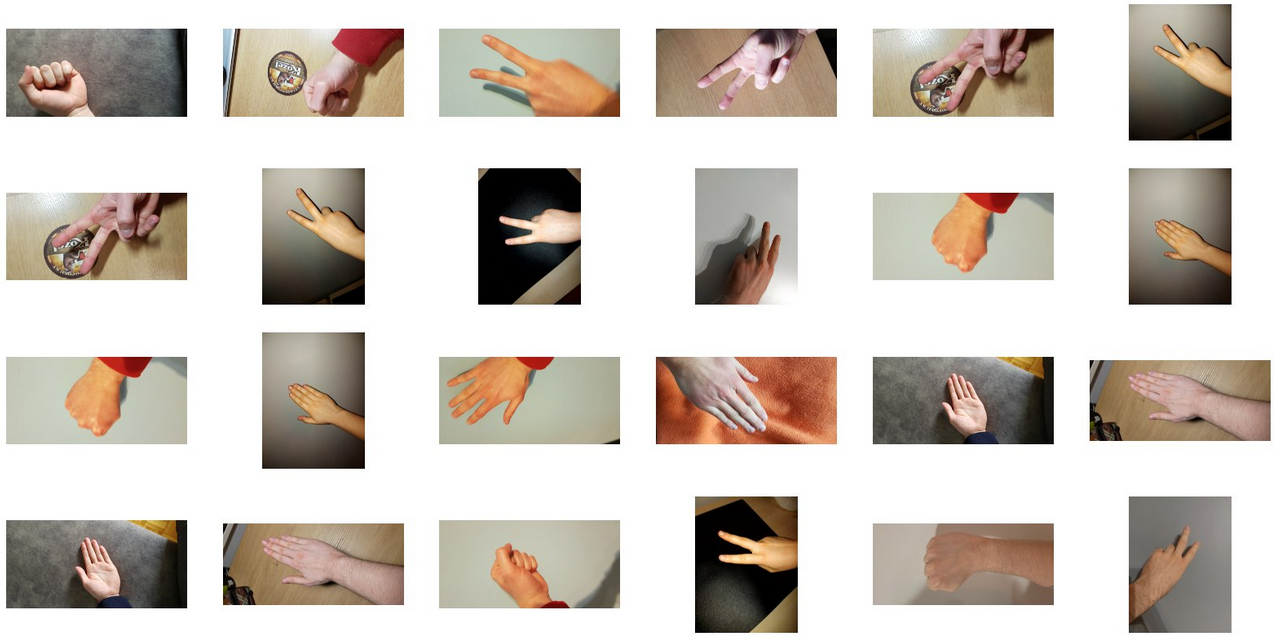
\includegraphics[scale=0.25]{images/self.png}
\end{frame}




\begin{frame}
  \frametitle{Self-made photos of hands}

  \begin{table}
    \centering
    \begin{tabular}{|c|c|}
    \hline
      \textbf{Model} & \textbf{Score} \\
      \hline
      KNN & 48.33\% \\
      \hline
      Decision tree & 45.00\% \\
      \hline
      Random forest & 46.66\% \\
      \hline
      XGBoost & 52.50\% \\
      \hline
      Support Vector Machine & 57.50\% \\
      \hline
    \end{tabular}
  \end{table}
  
\end{frame}








% \begin{frame}
%   \frametitle{Self-made photos of hands}
%   
\includegraphics[scale=0.25]{images/rasizm.png}
  

% \end{frame}










\begin{frame}
\centering

\includegraphics[height = \textheight]{images/michal.png}
% 
\includegraphics[angle=-90, width=\textwidth]{images/michal.png}
\end{frame}




\end{document}